\chapter*{LAMPIRAN}

\newappendix{Dokumentasi}

\begin{figure}[!h]
    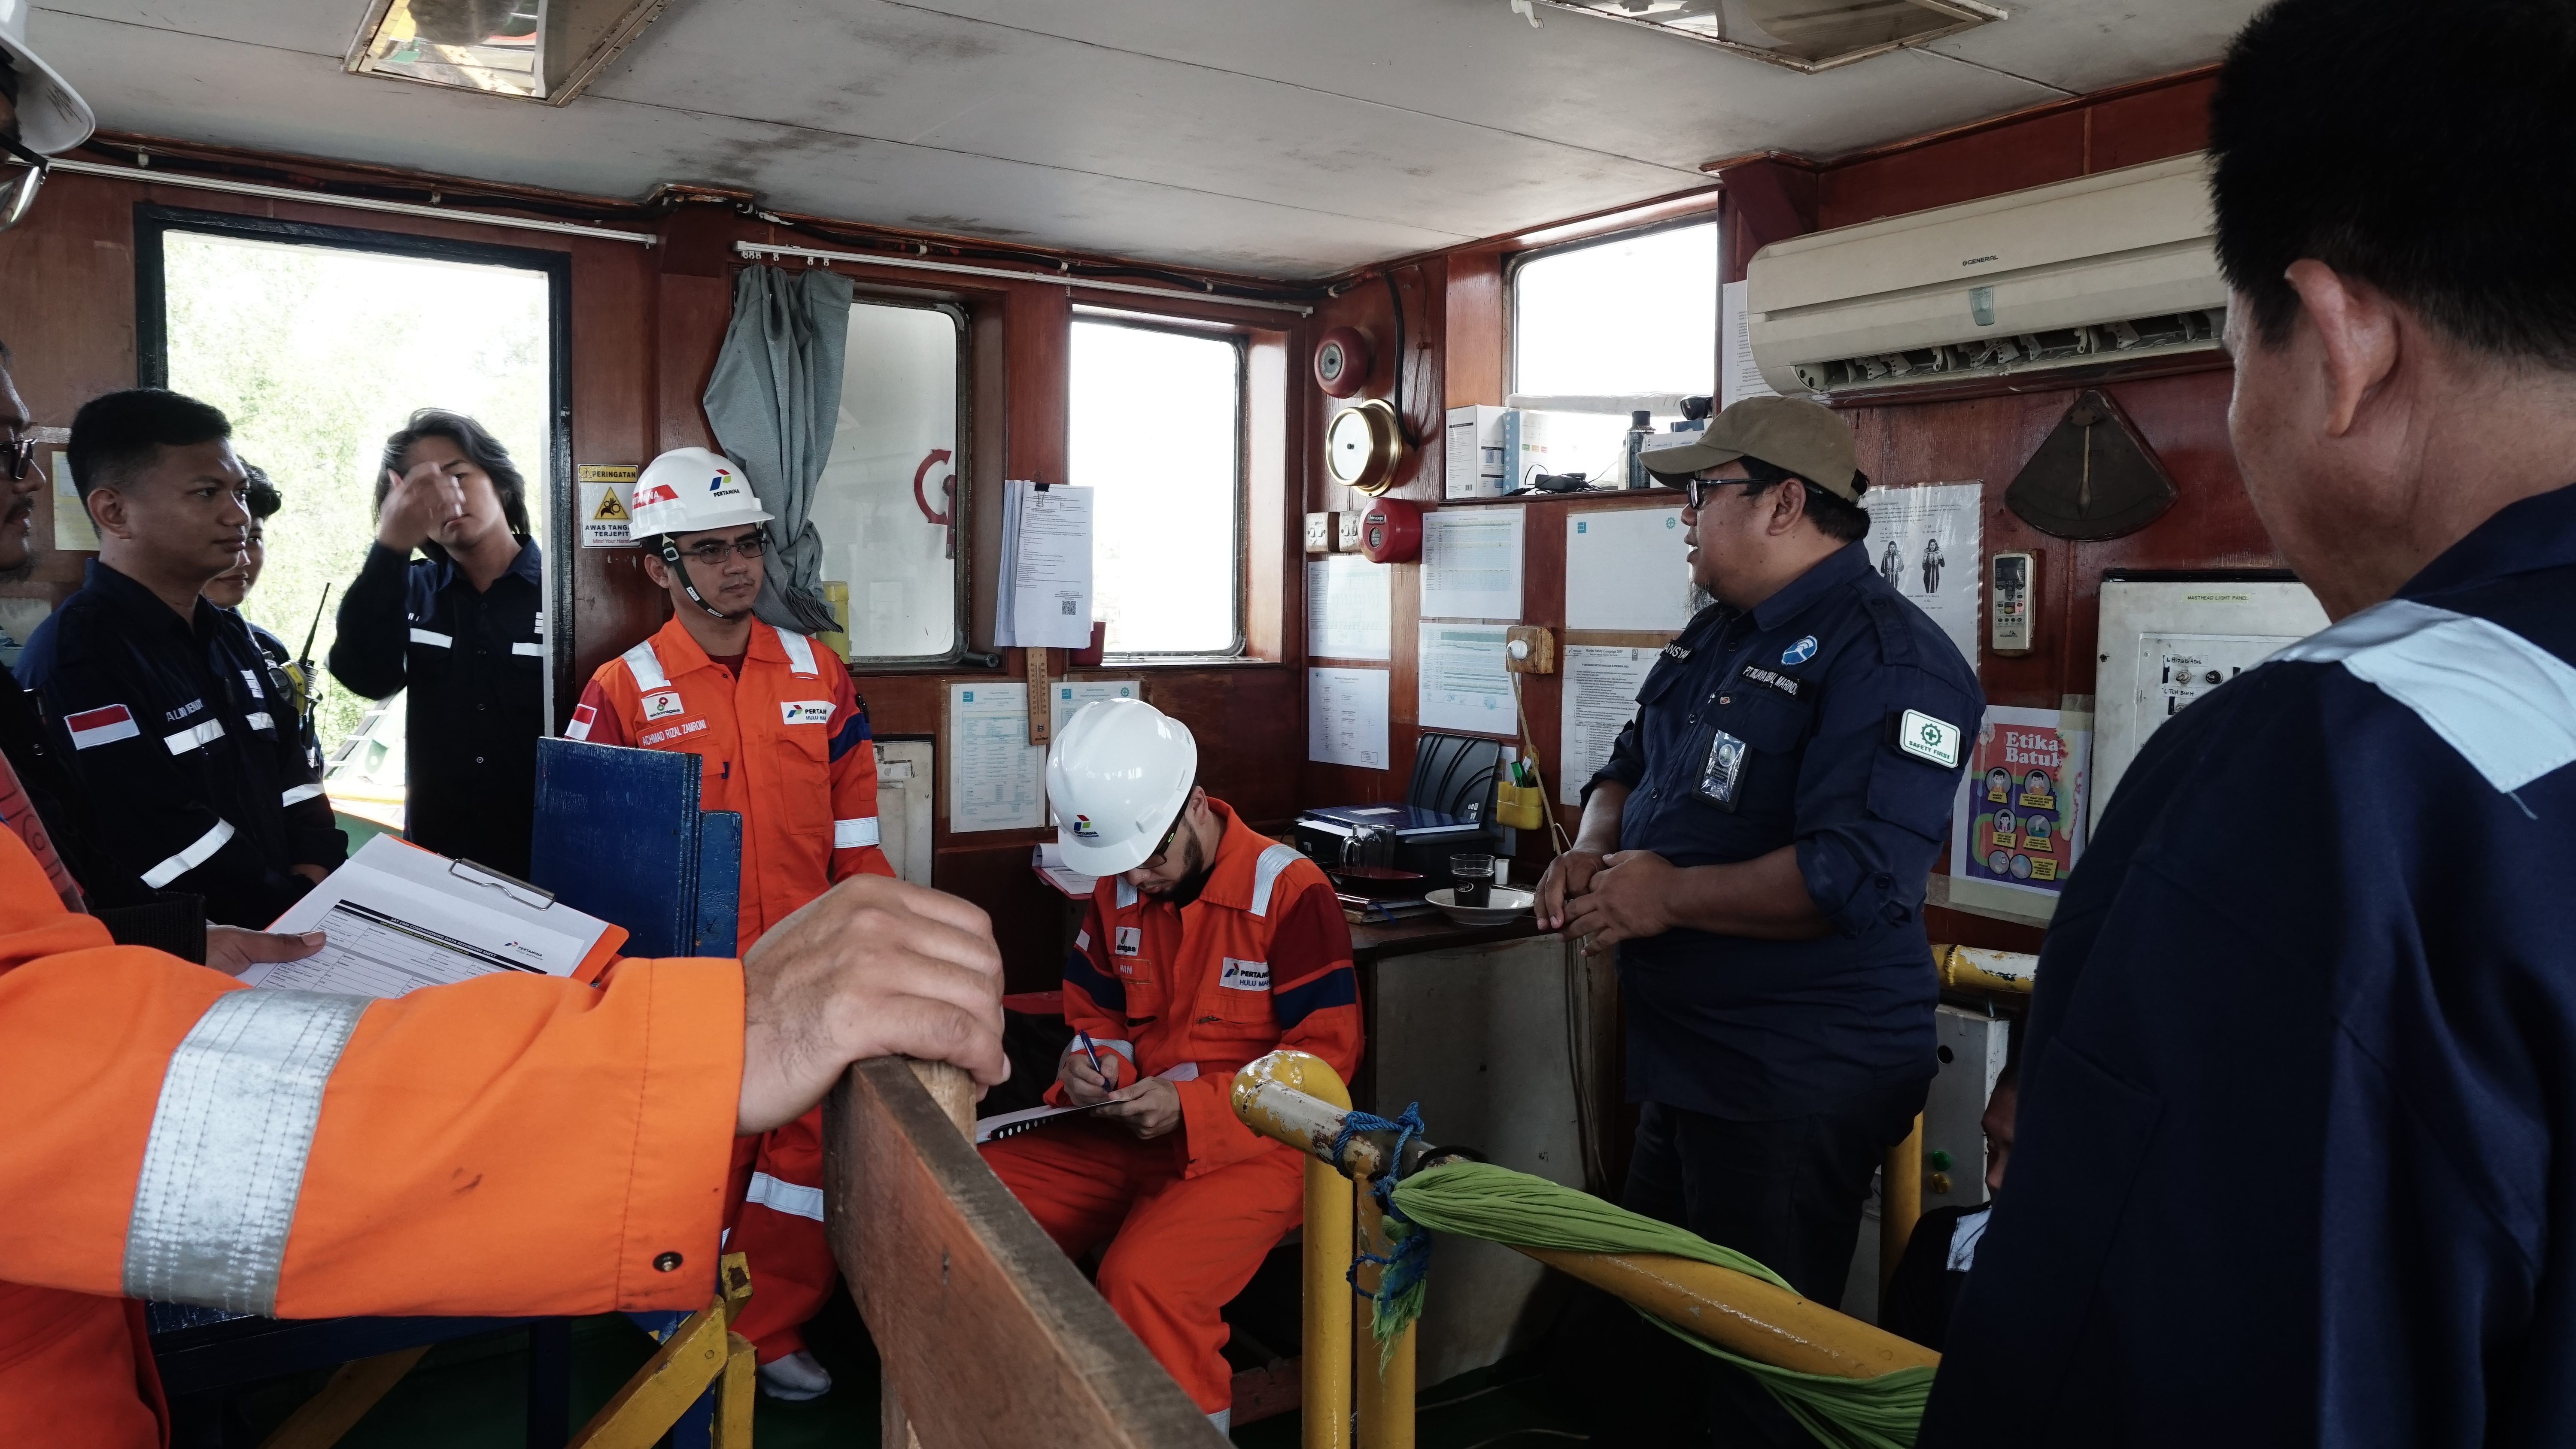
\includegraphics[width=.9\linewidth, center]{images/lampiran/documentation/validation.JPG}
    \caption{Validasi akurasi pembacaan sensor oleh mitra dan pihak ketiga}
    \label{fig:doc-validation}
\end{figure}

\begin{figure}[!h]
    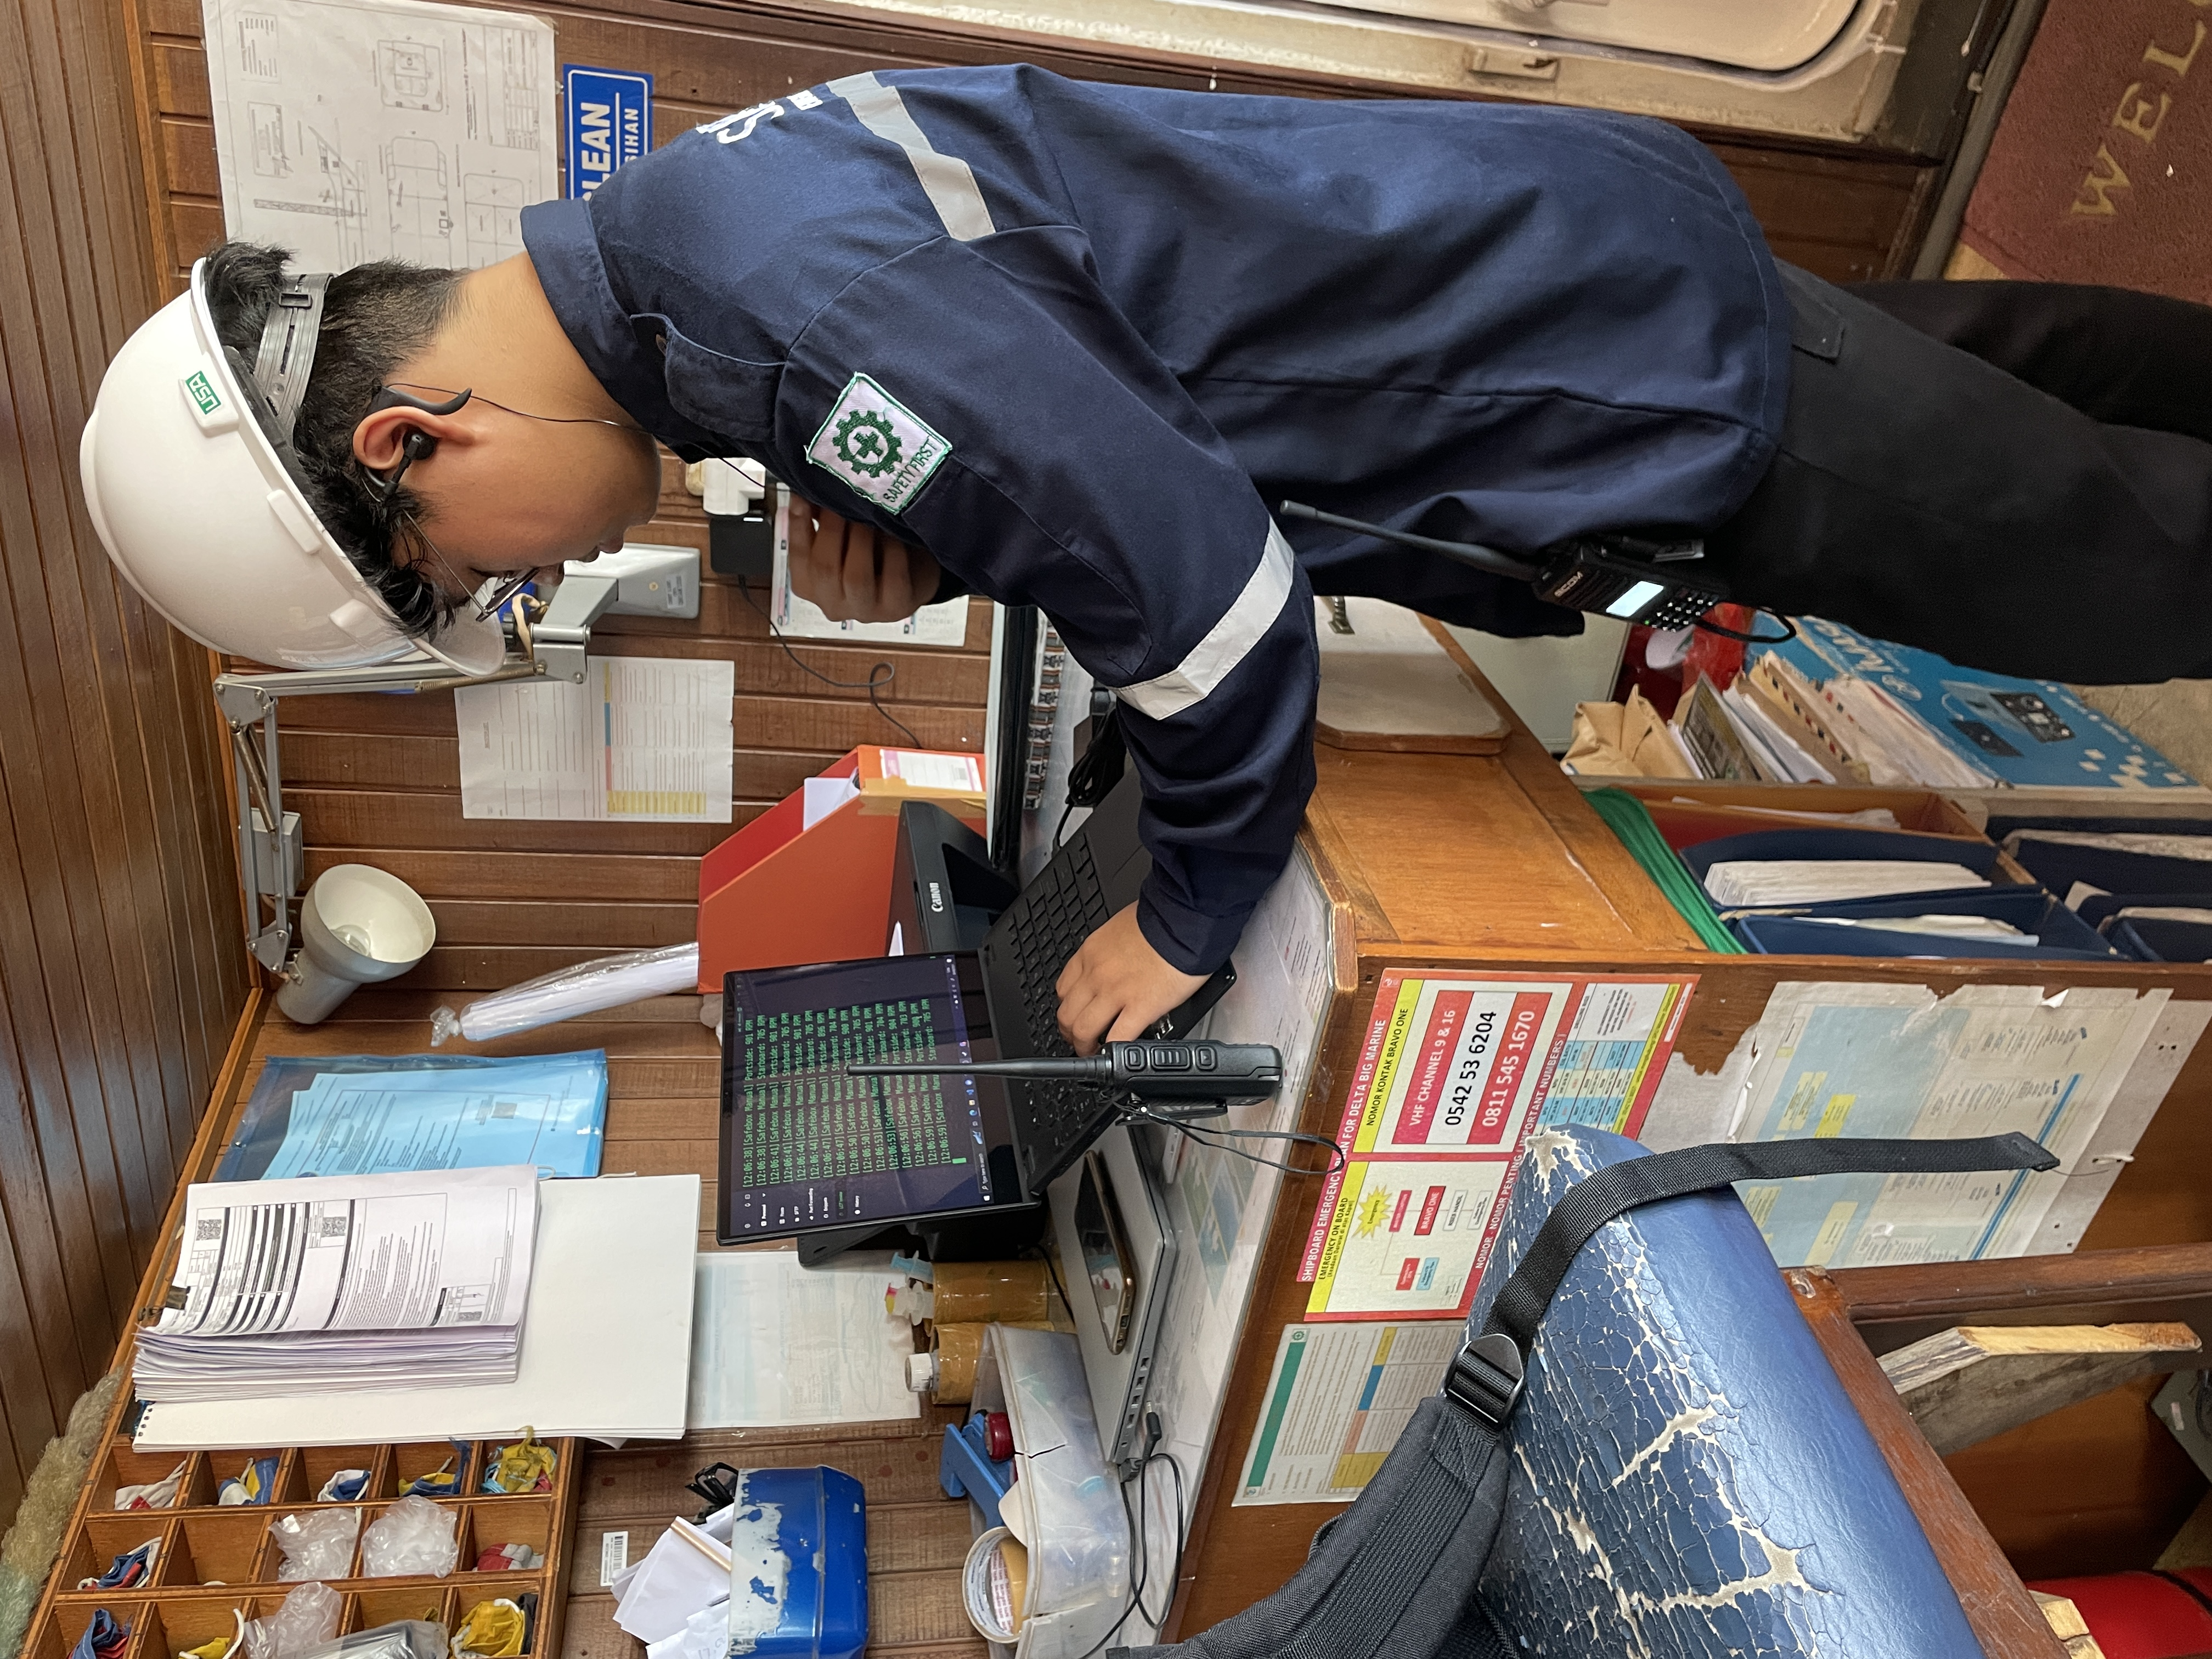
\includegraphics[angle=270, width=.5\linewidth, center]{images/lampiran/documentation/on-field.JPG}
    \caption{Pemasangan dan pengujian alat di lapangan}
    \label{fig:doc-lapangan}
\end{figure}

\begin{landscape}
    \newappendix{Hasil Implementasi}

    \subsection{Kebutuhan Fungsional}

    \begin{figure}[!h]
        \includegraphics[width=.6\linewidth, center]{images/lampiran/fr/fr-it1.png}
        \caption{Kebutuhan Fungsional Iterasi 1}
        \label{fig:fr-it1}
    \end{figure}

    \begin{figure}[!h]
        \includegraphics[width=1.1\linewidth, center]{images/lampiran/fr/fr-it2.png}
        \caption{Kebutuhan Fungsional Iterasi 2}
        \label{fig:fr-it2}
    \end{figure}

    \begin{figure}[!h]
        \includegraphics[width=1\linewidth, center]{images/lampiran/fr/fr-it3.png}
        \caption{Kebutuhan Fungsional Iterasi 3}
        \label{fig:fr-it3}
    \end{figure}

    \begin{figure}[!h]
        \includegraphics[width=1\linewidth, center]{images/lampiran/fr/fr-it4.png}
        \caption{Kebutuhan Fungsional Iterasi 4}
        \label{fig:fr-it4}
    \end{figure}

    \begin{figure}[!h]
        \includegraphics[width=1\linewidth, center]{images/lampiran/fr/fr-it5.png}
        \caption{Kebutuhan Fungsional Iterasi 5}
        \label{fig:fr-it5}
    \end{figure}

    \newpage
    \subsection{Wireframe}

    \begin{figure}[!h]
        \includegraphics[width=.7\linewidth, center]{images/lampiran/wireframe/wire-it1.png}
        \caption{Wireframe Iterasi 1}
        \label{fig:wire-it1}
    \end{figure}

    \begin{figure}[!h]
        \includegraphics[width=.7\linewidth, center]{images/lampiran/wireframe/wire-it2.png}
        \caption{Wireframe Iterasi 2}
        \label{fig:wire-it2}
    \end{figure}

    \begin{figure}[!h]
        \includegraphics[width=1\linewidth, center]{images/lampiran/wireframe/wire-it4.png}
        \caption{Wireframe Iterasi 4}
        \label{fig:wire-it4}
    \end{figure}

    \begin{figure}[!h]
        \includegraphics[width=.7\linewidth, center]{images/lampiran/wireframe/wire-it5.png}
        \caption{Wireframe Iterasi 5}
        \label{fig:wire-it5}
    \end{figure}

    \newpage

    \subsection{Coding}\label{apdx:coding}

    \begin{figure}[!h]
        \includegraphics[width=.8\linewidth, center]{images/lampiran/coding/code-it1.png}
        \caption{Coding Iterasi 1}
        \label{fig:code-it1}
    \end{figure}

    \begin{figure}[!h]
        \includegraphics[width=.85\linewidth, center]{images/lampiran/coding/code-it2.png}
        \caption{Coding Iterasi 2}
        \label{fig:code-it2}
    \end{figure}

    \begin{figure}[!h]
        \includegraphics[width=1\linewidth, center]{images/lampiran/coding/code-it5.png}
        \caption{Coding Iterasi 5}
        \label{fig:code-it5}
    \end{figure}

\end{landscape}

\newpage

\subsection{Whitebox Testing}\label{apdx:whitebox}

\begin{enumerate}
    \item Halaman Overview

    Backend: \href{https://github.com}{Link coming soon} \\
    Frontend: \href{https://github.com}{Link coming soon}

    \item Halaman Engine Speed

    Backend: \href{https://github.com}{Link coming soon} \\
    Frontend: \href{https://github.com}{Link coming soon}

    \item Halaman Fuel Consumption

    Backend: \href{https://github.com}{Link coming soon} \\
    Frontend: \href{https://github.com}{Link coming soon}

    \item Halaman OP41 Report

    Backend: \href{https://github.com}{Link coming soon} \\
    Frontend: \href{https://github.com}{Link coming soon}

    \item Halaman Running Hour

    Backend: \href{https://github.com}{Link coming soon} \\
    Frontend: \href{https://github.com}{Link coming soon}

    \item Halaman Data Log

    Backend: \href{https://github.com}{Link coming soon} \\
    Frontend: \href{https://github.com}{Link coming soon}
\end{enumerate}

\begin{landscape}
    \subsection{Blackbox Testing}

    \subsubsection{Iterasi 1}
    \begin{longtable}[!h]
    {
            p{0.2\textwidth}
            p{0.3\textwidth}
            p{0.3\textwidth}
            p{0.3\textwidth}
            p{0.3\textwidth}
            p{0.15\textwidth}
    }
    \caption{Blackbox Testing Halaman Engine Speed}
    \label{tab:it1-blackbox-es} \\

    \hline
        \bfseries \textit{Test Code} &
        \bfseries \textit{Test Case} &
        \bfseries \textit{Test Steps} &
        \bfseries \textit{Expected Result} &
        \bfseries \textit{Actual Result} &
        \bfseries \textit{Pass/Fail} \\ [0.5ex]
    \hline

    \endfirsthead

    \hline
        \bfseries \textit{Test Code} &
        \bfseries \textit{Test Case} &
        \bfseries \textit{Test Steps} &
        \bfseries \textit{Expected Result} &
        \bfseries \textit{Actual Result} &
        \bfseries \textit{Pass/Fail} \\ [0.5ex]
    \hline
    \endhead % all the lines above this will be repeated on every page
    \hline

    \csvreader[
        late after line=\\,
        before reading={\catcode`\#=12},after reading={\catcode`\#=6}
    ]{tables/hasil/iterations/1/blackbox/engine-speed.csv}
    {1=\code, 2=\case, 3=\step, 4=\expect, 5=\actual, 6=\status}
    {\code & \case & \step & \expect & \actual & \status} \\

    \bottomrule
\end{longtable}
    \newpage
    \subsubsection{Iterasi 2}
    \input{tables/hasil/iterations/2/blackbox/fuel-cons.tex}
    \newpage
    \input{tables/hasil/iterations/2/blackbox/running-hour.tex}
    \begin{longtable}[!h]
    {
            p{0.2\textwidth}
            p{0.3\textwidth}
            p{0.3\textwidth}
            p{0.3\textwidth}
            p{0.3\textwidth}
            p{0.15\textwidth}
    }
    \caption{Blackbox Testing Halaman Data Log}
    \label{tab:it1-blackbox-dl} \\

    \hline
        \bfseries \textit{Test Code} &
        \bfseries \textit{Test Case} &
        \bfseries \textit{Test Steps} &
        \bfseries \textit{Expected Result} &
        \bfseries \textit{Actual Result} &
        \bfseries \textit{Pass/Fail} \\ [0.5ex]
    \hline

    \endfirsthead

    \hline
        \bfseries \textit{Test Code} &
        \bfseries \textit{Test Case} &
        \bfseries \textit{Test Steps} &
        \bfseries \textit{Expected Result} &
        \bfseries \textit{Actual Result} &
        \bfseries \textit{Pass/Fail} \\ [0.5ex]
    \hline
    \endhead % all the lines above this will be repeated on every page
    \hline

    \csvreader[
        late after line=\\,
        before reading={\catcode`\#=12},after reading={\catcode`\#=6}
    ]{tables/hasil/iterations/2/blackbox/data-log.csv}
    {1=\code, 2=\case, 3=\step, 4=\expect, 5=\actual, 6=\status}
    {\code & \case & \step & \expect & \actual & \status} \\

    \bottomrule
\end{longtable}
    \subsubsection{Iterasi 3}
    \input{tables/hasil/iterations/3/blackbox/fcrv.tex}
    \input{tables/hasil/iterations/3/blackbox/user.tex}
    \newpage
    \input{tables/hasil/iterations/3/blackbox/vessel.tex}
    \input{tables/hasil/iterations/3/blackbox/fcrv.tex}
    \input{tables/hasil/iterations/3/blackbox/fcrv.tex}
    \newpage
    \subsubsection{Iterasi 4}
    \input{tables/hasil/iterations/4/blackbox/generate-es-report.tex}
    \newpage
    \input{tables/hasil/iterations/4/blackbox/generate-fuel-report.tex}
    \newpage
    \subsubsection{Iterasi 5}
    \input{tables/hasil/iterations/5/blackbox/export-data.tex}

\end{landscape}

% \section{\textit{Source Code}}

% \begin{enumerate}
%     \item \href{https://github.com}{Frontend Halaman Engine Speed}
%     \item \href{https://github.com}{Frontend Halaman Overview}
%     \item \href{https://github.com}{Frontend Halaman Fuel Consumption}
%     \item \href{https://github.com}{Frontend Halaman OP41 Report}
%     \item \href{https://github.com}{Frontend Halaman Running Hour}
%     \item \href{https://github.com}{Frontend Halaman Data Log}
%     \item \href{https://github.com}{Backend Overview}
%     \item \href{https://github.com}{Backend Engine Speed}
%     \item \href{https://github.com}{Backend Halaman Fuel Consumption}
%     \item \href{https://github.com}{Backend Halaman OP41 Report}
%     \item \href{https://github.com}{Backend Halaman Running Hour}
%     \item \href{https://github.com}{Backend Halaman Data Log}
% \end{enumerate}